\documentclass[E:/Latex/ExtraWork/ComputerArchitechture/Report.tex]{subfiles}
\usepackage[utf8]{inputenc}
\PassOptionsToPackage{english, british}{babel}
\usepackage[english, british]{babel}
\usepackage{graphicx}
\graphicspath{{../ComputerArchitechture/Chapter1/Figure/}}
\usepackage{amsmath}
\usepackage{amsfonts}
\usepackage{multirow}
\usepackage{booktabs}
\usepackage{indentfirst}
\usepackage{tabularx}
\usepackage{amssymb}
\usepackage{setspace}		%use \doublespacing
\begin{document}
	\pagenumbering{arabic}
	\setcounter{page}{1}
	% \begin{otherlanguage}{english}
		\chapter{Cơ sở lý thuyết về CPU RICSV 32}
			\section{Giới thiệu tổng quát về CPU RICSV 32}

	CPU RICSV 32 có tổng cộng 32 lệnh hợp ngữ, mỗi lệnh có độ dài 32 bits và 7 bits [6:0] (opcode) để xác định loại lệnh.	
		
						
	Tập lệnh của RICSV 32 còn được gọi là tập lệnh kiểu load-store, nghĩa là data trong bộ nhớ muốn được thực thi thì trước hết phải được lấy ra bỏ vào băng thanh ghi rồi mới được tính toán. Sau khi tính toán, data sẽ được lưu lại vào memory.	
							
	Các thanh ghi trong băng thanh ghi (Register Bank) có độ dài 32 bits và có 32 thanh ghi (từ $x_0 - x_{31}$), cần có 5 bits để xác định địa chỉ của các thanh ghi trong băng thanh ghi. Trong đó, chức năng của 32 thanh ghi được cho như bảng bên dưới.  	

				\begin{table}[!ht]
				\begin{center}
				\begin{tabular}{|c|c|c|c|}
					\hline
					\multicolumn{1}{|l|}{\textbf {Register}} & \multicolumn{1}{l|}{\textbf {ABI name}} & \multicolumn{1}{l|}{\textbf {Description}}  & \multicolumn{1}{l|}{\textbf {Saver}} \\ 
					\hline
					x0                             & zero                          & Hard-wired zero                   & \_\_\_                     \\
					x1                             & ra                            & Return address                    & Caller                     \\
					x2                             & sp                            & Stack pointer                     & Caller                     \\
					x3                             & gp                            & Global pointer                    & \_\_\_                     \\
					x4                             & tp                            & Thread pointer                    & \_\_\_                     \\
					x5                             & t0                            & Temporary/alternate link register & Caller                     \\
					x6-7                           & t1-2                          & Temporaries                       & Caller                     \\
					x8                             & s0/fp                         & Saved register/frame pointer      & Caller                     \\
					x9                             & s1                            & Saved register                    & Caller                     \\
					x10-11                         & a0-1                          & Function arguments/return values  & Caller                     \\
					x12-17                         & a2-7                          & Function arguments                & Caller                     \\
					x18-27                         & s2-11                         & Saved registers                   & Caller                     \\
					x28-31                         & t3-6                          & Temporaries                       & Caller                     \\ 
					\hline 
					\end{tabular}
					\end{center}
					\end{table}
	\textbf {\underline{Lưu ý:} Thanh ghi $x_0$ luôn có giá trị bằng 0x000000000 và không thay đổi giá trị này.}
							
	Dữ liệu trong cả bộ nhớ dữ liệu (DMEM) và bộ nhớ chương trình (IMEM) đều có độ dài 32bit và được sắp xếp theo kiểu \textbf {little edian}.
							
	DMEM được định địa chỉ theo từng byte ( = 8 bits) chứ không theo word ( = 32 bits). Nếu định địa chỉ theo word thì lấy địa chỉ của byte có trọng số thấp nhất.
							
	Điều này được trình bày như ở hình dưới.
			\begin{figure}[h!]
				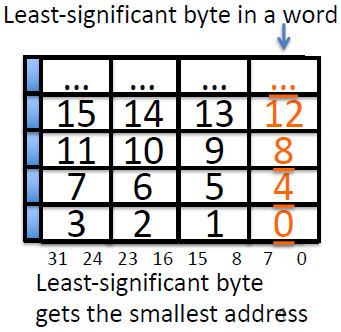
\includegraphics[scale = 0.7]{Figure/Fig2.png}
				\centering
			\end{figure}	
	\newpage

\section{Nhóm lệnh R-Format}
	Nhóm lệnh này bao gồm các lệnh có cấu trúc như ở hình sau:

	\begin{figure}[h!]
				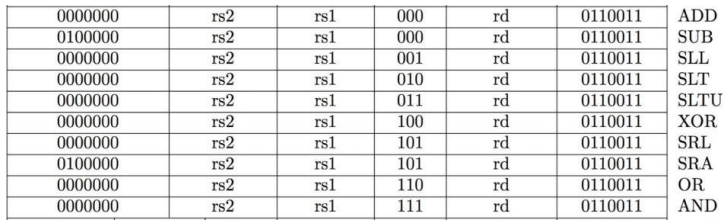
\includegraphics[scale = 0.9]{Figure/Fig3.png}
				\centering
			\end{figure}	

	Nhóm lệnh này có opcode là [6:0] = 0110011

	Nhóm lệnh này thực hiện lấy hai giá trị lưu ở thanh ghi \textbf{rs1} và \textbf{rs2} thực hiện đưa vào khối ALU để tính toán, sau đó lưu kết quả vào thanh ghi \textbf{rd}.

\section{Nhóm lệnh I (tính toán)}
			
			\begin{figure}[h!]
				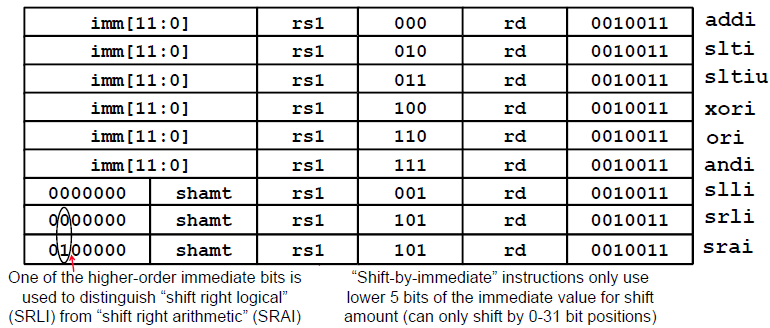
\includegraphics[scale = 0.9]{Figure/Fig4.png}
				\centering
			\end{figure}	

	Nhóm lệnh này có opcode là [6:0] = 0010011

	Nhóm lệnh này (trừ 3 lệnh SRAI, SRLI, SLLI) thực hiện lấy giá trị lưu ở thanh ghi \textbf{rs1} và giá trị lưu ở \textbf{imm[11:0]} (được mở rộng dấu), thực hiện đưa vào khối ALU để tính toán. Kết quả được lưu vào thanh ghi \textbf{rd}.
	\newpage

\section{Nhóm lệnh L (Load data)}
			\begin{figure}[h!]
				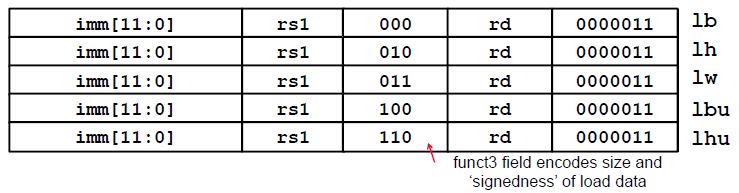
\includegraphics[scale = 0.9]{Figure/Fig5.png}
				\centering
			\end{figure}	
	Nhóm lệnh này có opcode là [6:0] = 0000011

	Nhóm lệnh này thực hiện lấy hai giá trị lưu ở thanh ghi \textbf{rs1} và giá trị lưu ở \textbf{imm[11:0]} (được mở rộng dấu) để tính tổng \textbf{rs1 + ext(imm[11:0])}. Sau đó lấy giá trị lưu trong DMEM tại địa chỉ \textbf{rs1 + ext(imm[11:0])}, lưu vào thanh ghi \textbf{rd}.

\section{Nhóm lệnh S (Store data)}
			\begin{figure}[h!]
				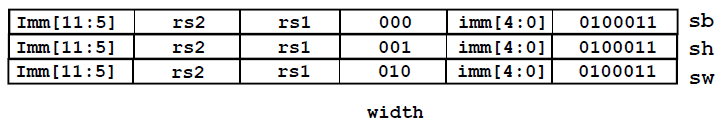
\includegraphics[scale = 0.9]{Figure/Fig6.png}
				\centering
			\end{figure}	
	Nhóm lệnh này có opcode là [6:0] = 0100011

	Nhóm lệnh này thực hiện lấy hai giá trị lưu ở thanh ghi \textbf{rs1} và giá trị lưu ở \textbf{imm[11:5]} và \textbf{imm[4:0]} (ghép lại và mở rộng dấu) để tính tổng \textbf{rs1 + ext(imm[11:5])imm[4:0]}. Sau đó lấy giá trị lưu trong thanh ghi \textbf{rs2} lưu vào DMEM tại địa chỉ \textbf {rs1 + ext(imm[11:5]imm[4:0])}.

\section{Nhóm lệnh B (Rẽ nhánh)}
		\begin{figure}[h!]
			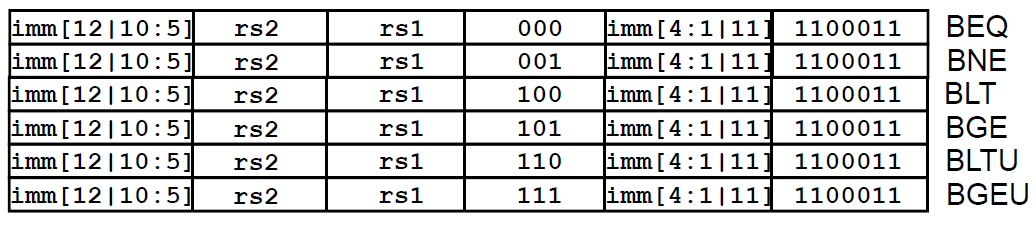
\includegraphics[scale = 0.7]{Figure/Fig7.png}
			\centering
		\end{figure}
	Nhóm lệnh này có opcode là [6:0] = 1100011

	Nhóm lệnh này sẽ thực hiện chuyển giá trị của thanh ghi PC thành giá trị được lưu trong các phần \textbf{imm} giá trị lưu trong \textbf{rs1} và \textbf{rs2} thỏa điều kiện câu lệnh (bằng, không bằng, lớn hơn hoặc bằng,…). 

	Khi lấy giá trị lưu ở phần \textbf{imm} ta phải ghép lại cho đúng thứ tự và mở rộng dấu, bit LSB luôn luôn bằng 0.

	Lấy ví dụ như ở hình dưới:
			\begin{figure}[h!]
				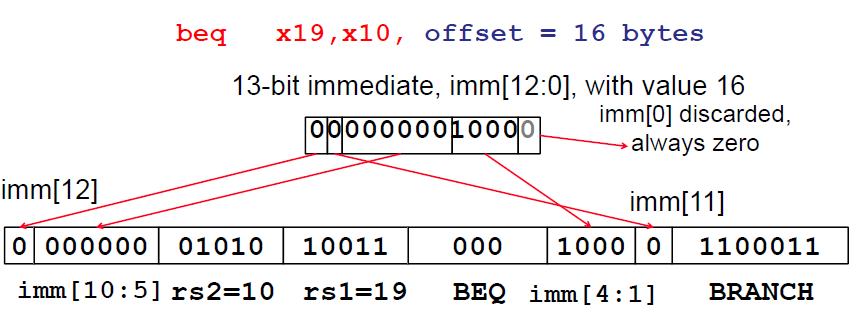
\includegraphics[scale = 0.7]{Figure/Fig8.png}
				\centering
			\end{figure}


\section{Nhóm lệnh U}
			\begin{figure}[h!]
					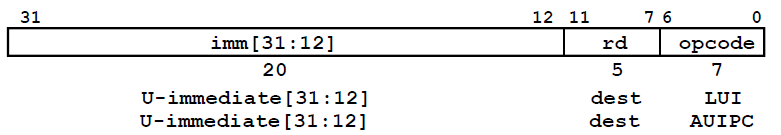
\includegraphics[scale = 0.7]{Figure/Fig9.png}
					\centering
			\end{figure}

	Với lệnh LUI
	 	\begin{itemize}
	 		\item Opcode = 0110111
	 		\item Lệnh này load giá trị \textbf {imm[31:12]00000000000} vào thanh ghi \textbf {rd}.
	 	\end{itemize}
	 	
	Với lệnh AUIPC
	 	\begin{itemize}
	 		\item Opcode = 0010111
	 		\item Lệnh này load giá trị ở \textbf{PC} vào thanh ghi \text{rd}.
	 	\end{itemize}
\section{Nhóm lệnh J (nhảy không điều kiện)}
	\begin{figure}[h!]
					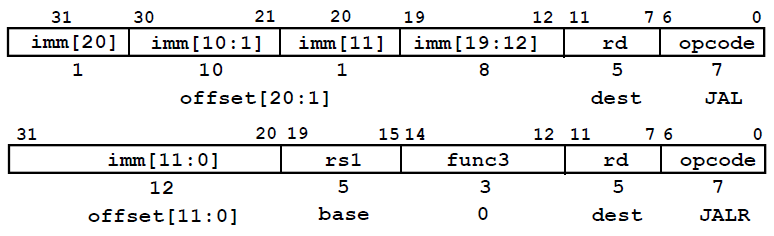
\includegraphics[scale = 0.7]{Figure/Fig10.png}
					\centering
			\end{figure}
	% \end{otherlanguage}

\end{document}